% GNUPLOT: LaTeX picture with Postscript
\begingroup
  \makeatletter
  \providecommand\color[2][]{%
    \GenericError{(gnuplot) \space\space\space\@spaces}{%
      Package color not loaded in conjunction with
      terminal option `colourtext'%
    }{See the gnuplot documentation for explanation.%
    }{Either use 'blacktext' in gnuplot or load the package
      color.sty in LaTeX.}%
    \renewcommand\color[2][]{}%
  }%
  \providecommand\includegraphics[2][]{%
    \GenericError{(gnuplot) \space\space\space\@spaces}{%
      Package graphicx or graphics not loaded%
    }{See the gnuplot documentation for explanation.%
    }{The gnuplot epslatex terminal needs graphicx.sty or graphics.sty.}%
    \renewcommand\includegraphics[2][]{}%
  }%
  \providecommand\rotatebox[2]{#2}%
  \@ifundefined{ifGPcolor}{%
    \newif\ifGPcolor
    \GPcolortrue
  }{}%
  \@ifundefined{ifGPblacktext}{%
    \newif\ifGPblacktext
    \GPblacktexttrue
  }{}%
  % define a \g@addto@macro without @ in the name:
  \let\gplgaddtomacro\g@addto@macro
  % define empty templates for all commands taking text:
  \gdef\gplbacktext{}%
  \gdef\gplfronttext{}%
  \makeatother
  \ifGPblacktext
    % no textcolor at all
    \def\colorrgb#1{}%
    \def\colorgray#1{}%
  \else
    % gray or color?
    \ifGPcolor
      \def\colorrgb#1{\color[rgb]{#1}}%
      \def\colorgray#1{\color[gray]{#1}}%
      \expandafter\def\csname LTw\endcsname{\color{white}}%
      \expandafter\def\csname LTb\endcsname{\color{black}}%
      \expandafter\def\csname LTa\endcsname{\color{black}}%
      \expandafter\def\csname LT0\endcsname{\color[rgb]{1,0,0}}%
      \expandafter\def\csname LT1\endcsname{\color[rgb]{0,1,0}}%
      \expandafter\def\csname LT2\endcsname{\color[rgb]{0,0,1}}%
      \expandafter\def\csname LT3\endcsname{\color[rgb]{1,0,1}}%
      \expandafter\def\csname LT4\endcsname{\color[rgb]{0,1,1}}%
      \expandafter\def\csname LT5\endcsname{\color[rgb]{1,1,0}}%
      \expandafter\def\csname LT6\endcsname{\color[rgb]{0,0,0}}%
      \expandafter\def\csname LT7\endcsname{\color[rgb]{1,0.3,0}}%
      \expandafter\def\csname LT8\endcsname{\color[rgb]{0.5,0.5,0.5}}%
    \else
      % gray
      \def\colorrgb#1{\color{black}}%
      \def\colorgray#1{\color[gray]{#1}}%
      \expandafter\def\csname LTw\endcsname{\color{white}}%
      \expandafter\def\csname LTb\endcsname{\color{black}}%
      \expandafter\def\csname LTa\endcsname{\color{black}}%
      \expandafter\def\csname LT0\endcsname{\color{black}}%
      \expandafter\def\csname LT1\endcsname{\color{black}}%
      \expandafter\def\csname LT2\endcsname{\color{black}}%
      \expandafter\def\csname LT3\endcsname{\color{black}}%
      \expandafter\def\csname LT4\endcsname{\color{black}}%
      \expandafter\def\csname LT5\endcsname{\color{black}}%
      \expandafter\def\csname LT6\endcsname{\color{black}}%
      \expandafter\def\csname LT7\endcsname{\color{black}}%
      \expandafter\def\csname LT8\endcsname{\color{black}}%
    \fi
  \fi
    \setlength{\unitlength}{0.0500bp}%
    \ifx\gptboxheight\undefined%
      \newlength{\gptboxheight}%
      \newlength{\gptboxwidth}%
      \newsavebox{\gptboxtext}%
    \fi%
    \setlength{\fboxrule}{0.5pt}%
    \setlength{\fboxsep}{1pt}%
\begin{picture}(14400.00,5760.00)%
    \gplgaddtomacro\gplbacktext{%
      \csname LTb\endcsname%%
      \put(618,624){\makebox(0,0)[r]{\strut{}0.0}}%
      \csname LTb\endcsname%%
      \put(618,1296){\makebox(0,0)[r]{\strut{}2.0}}%
      \csname LTb\endcsname%%
      \put(618,1969){\makebox(0,0)[r]{\strut{}4.0}}%
      \csname LTb\endcsname%%
      \put(618,2641){\makebox(0,0)[r]{\strut{}6.0}}%
      \csname LTb\endcsname%%
      \put(618,3313){\makebox(0,0)[r]{\strut{}8.0}}%
      \csname LTb\endcsname%%
      \put(618,3985){\makebox(0,0)[r]{\strut{}10.0}}%
      \csname LTb\endcsname%%
      \put(618,4658){\makebox(0,0)[r]{\strut{}12.0}}%
      \csname LTb\endcsname%%
      \put(618,5330){\makebox(0,0)[r]{\strut{}14.0}}%
      \csname LTb\endcsname%%
      \put(720,102){\makebox(0,0){\strut{}$240$}}%
      \csname LTb\endcsname%%
      \put(1697,102){\makebox(0,0){\strut{}$250$}}%
      \csname LTb\endcsname%%
      \put(2674,102){\makebox(0,0){\strut{}$260$}}%
      \csname LTb\endcsname%%
      \put(3651,102){\makebox(0,0){\strut{}$270$}}%
      \csname LTb\endcsname%%
      \put(4628,102){\makebox(0,0){\strut{}$280$}}%
      \csname LTb\endcsname%%
      \put(5605,102){\makebox(0,0){\strut{}$290$}}%
      \csname LTb\endcsname%%
      \put(6582,102){\makebox(0,0){\strut{}$300$}}%
    }%
    \gplgaddtomacro\gplfronttext{%
      \csname LTb\endcsname%%
      \put(126,2977){\rotatebox{-270}{\makebox(0,0){\strut{}Absorbance / 1\,cm / \np{e-3}}}}%
      \csname LTb\endcsname%%
      \put(6975,3453){\makebox(0,0)[r]{\strut{}0.016\%}}%
      \csname LTb\endcsname%%
      \put(6975,3639){\makebox(0,0)[r]{\strut{}0.018\%}}%
      \csname LTb\endcsname%%
      \put(6975,3825){\makebox(0,0)[r]{\strut{}0.020\%}}%
      \csname LTb\endcsname%%
      \put(6975,4011){\makebox(0,0)[r]{\strut{}0.022\%}}%
      \csname LTb\endcsname%%
      \put(6975,4197){\makebox(0,0)[r]{\strut{}0.024\%}}%
      \csname LTb\endcsname%%
      \put(6975,4383){\makebox(0,0)[r]{\strut{}0.030\%}}%
      \csname LTb\endcsname%%
      \put(6975,4569){\makebox(0,0)[r]{\strut{}0.050\%}}%
      \csname LTb\endcsname%%
      \put(6975,4755){\makebox(0,0)[r]{\strut{}0.100\%}}%
      \csname LTb\endcsname%%
      \put(6975,4941){\makebox(0,0)[r]{\strut{}0.160\%}}%
      \csname LTb\endcsname%%
      \put(6975,5127){\makebox(0,0)[r]{\strut{}0.180\%}}%
      \csname LTb\endcsname%%
      \put(6975,5313){\makebox(0,0)[r]{\strut{}0.200\%}}%
      \csname LTb\endcsname%%
      \put(6975,5499){\makebox(0,0)[r]{\strut{}0.220\%}}%
    }%
    \gplgaddtomacro\gplbacktext{%
      \csname LTb\endcsname%%
      \put(7457,624){\makebox(0,0)[r]{\strut{}}}%
      \csname LTb\endcsname%%
      \put(7457,1296){\makebox(0,0)[r]{\strut{}}}%
      \csname LTb\endcsname%%
      \put(7457,1969){\makebox(0,0)[r]{\strut{}}}%
      \csname LTb\endcsname%%
      \put(7457,2641){\makebox(0,0)[r]{\strut{}}}%
      \csname LTb\endcsname%%
      \put(7457,3313){\makebox(0,0)[r]{\strut{}}}%
      \csname LTb\endcsname%%
      \put(7457,3985){\makebox(0,0)[r]{\strut{}}}%
      \csname LTb\endcsname%%
      \put(7457,4658){\makebox(0,0)[r]{\strut{}}}%
      \csname LTb\endcsname%%
      \put(7457,5330){\makebox(0,0)[r]{\strut{}}}%
      \csname LTb\endcsname%%
      \put(7559,102){\makebox(0,0){\strut{}$240$}}%
      \csname LTb\endcsname%%
      \put(8529,102){\makebox(0,0){\strut{}$250$}}%
      \csname LTb\endcsname%%
      \put(9499,102){\makebox(0,0){\strut{}$260$}}%
      \csname LTb\endcsname%%
      \put(10469,102){\makebox(0,0){\strut{}$270$}}%
      \csname LTb\endcsname%%
      \put(11438,102){\makebox(0,0){\strut{}$280$}}%
      \csname LTb\endcsname%%
      \put(12408,102){\makebox(0,0){\strut{}$290$}}%
      \csname LTb\endcsname%%
      \put(13378,102){\makebox(0,0){\strut{}$300$}}%
      \csname LTb\endcsname%%
      \put(14348,102){\makebox(0,0){\strut{}$310$}}%
      \csname LTb\endcsname%%
      \put(10954,4658){\makebox(0,0){\strut{}\shortstack{background \\ subtraction}}}%
    }%
    \gplgaddtomacro\gplfronttext{%
      \csname LTb\endcsname%%
      \put(7457,2977){\rotatebox{-270}{\makebox(0,0){\strut{}}}}%
    }%
    \gplbacktext
    \put(0,0){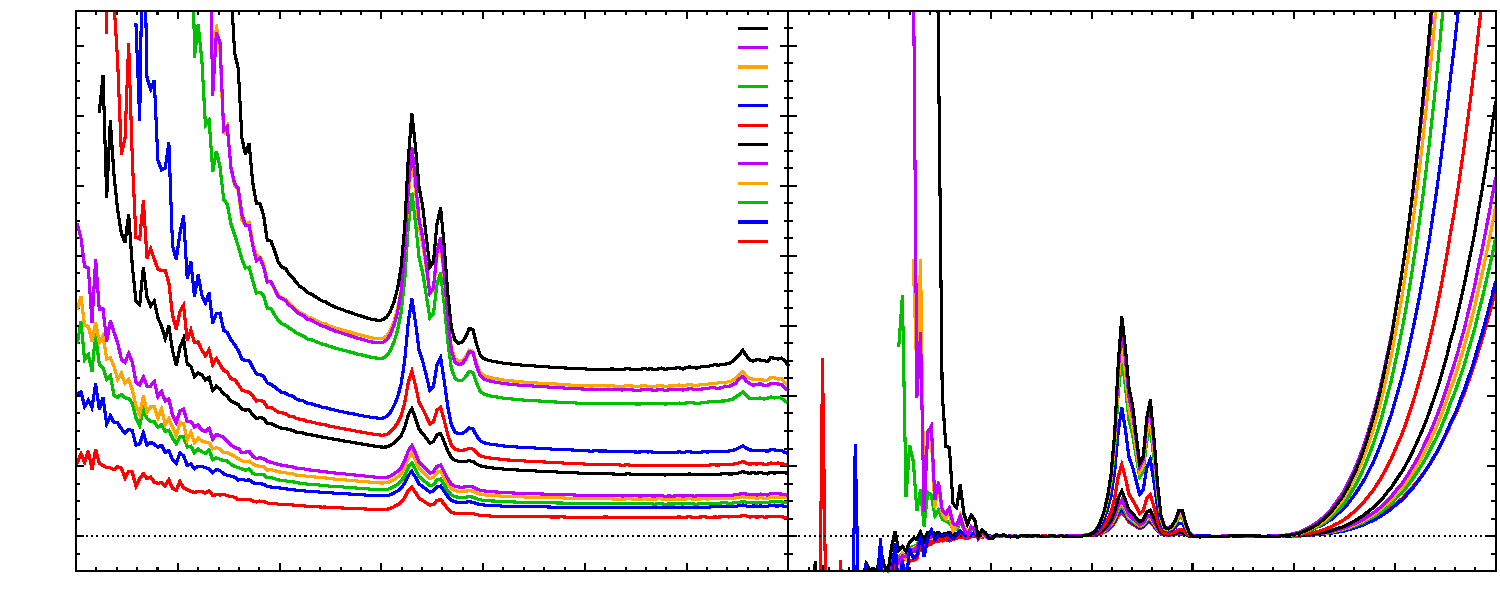
\includegraphics{pics/polyfit}}%
    \gplfronttext
  \end{picture}%
\endgroup
